% !TeX program = xelatex
\documentclass[fontset=fandol,12pt,a4paper]{ctexart}
% ---------- 正文字号（12pt -> 14pt，四号）----------
\usepackage[fontsize=14pt]{fontsize}
\usepackage[margin=2.54cm,headheight=22pt]{geometry}
\setlength{\emergencystretch}{2em}
\usepackage{amsmath,amssymb}
\usepackage{enumitem}
\usepackage{graphicx}
\usepackage{fancyhdr}
\usepackage[colorlinks,linkcolor=blue,citecolor=blue,urlcolor=blue]{hyperref}

% ---------- 页眉：左侧 QXC logo，右侧姓名与日期 ----------
\graphicspath{{logo/}{../logo/}}
\newcommand{\qxcLogo}{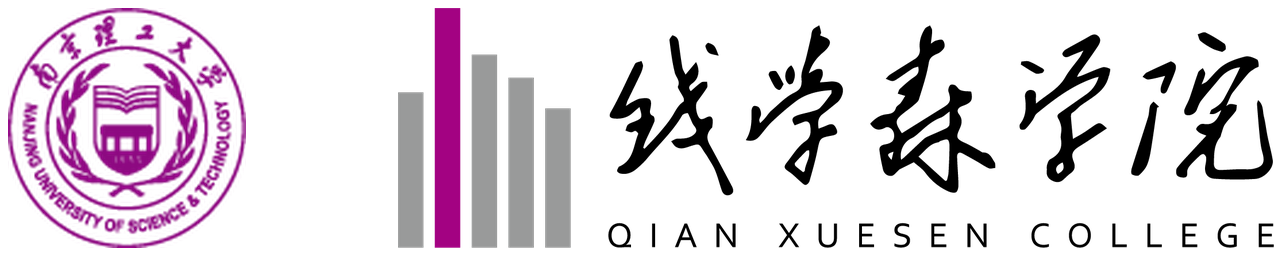
\includegraphics[height=0.6cm]{QXC.png}}
% 页眉右侧文字（改姓名或日期格式只需改这一行）
\newcommand{\qxcHeaderRight}{\small 魏舟\qquad\today}
\fancypagestyle{qxcheader}{%
	\fancyhf{}%
	\fancyhead[L]{\qxcLogo}%
	\fancyhead[R]{\qxcHeaderRight}%
	\fancyfoot[C]{\normalsize\thepage}%
	\renewcommand{\headrulewidth}{0.4pt}%
	\renewcommand{\footrulewidth}{0pt}%
}
\pagestyle{qxcheader}
% 标题页（plain 样式）用同一套页眉页脚
\fancypagestyle{plain}{%
	\fancyhf{}%
	\fancyhead[L]{\qxcLogo}%
	\fancyhead[R]{\qxcHeaderRight}%
	\fancyfoot[C]{\normalsize\thepage}%
	\renewcommand{\headrulewidth}{0.4pt}%
	\renewcommand{\footrulewidth}{0pt}%
}
\title{练习二}
% 姓名与日期已移到页眉（见上方 \qxcHeaderRight），此处留空以免与页眉重复
\author{}
\date{}
\begin{document}
\maketitle
\section{习题1.}
\begin{figure}[htbp]
  \centering
  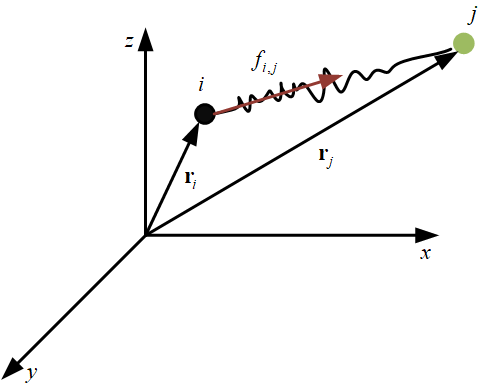
\includegraphics[width=0.5\linewidth]{figure/练习二习题1.png}
  \caption{示意图}
  \label{fig:1}
\end{figure}

设微元 $i$ 的位置为 $\boldsymbol{r}_{i}=[x_i,y_i,z_i]^{\mathrm{T}}$，

微元 $j$ 的位置为$\boldsymbol{r}_{j}=[x_j,y_j,z_j]^{\mathrm{T}}$，

则两微元之间的距离，
\begin{equation}
	\label{eq:dist}
	d_{i j}=\left|\boldsymbol{r}_{j}-\boldsymbol{r}_{i}\right| ,
\end{equation}
连接两微元的弹簧刚度为 $k$、原长为 $l$，弹性恢复力为
\begin{equation}
	\label{eq:springforce}
	\boldsymbol{f}_{i, j}=k\left(d_{i j}-l\right) \boldsymbol{n}_{i, j} ,
	\qquad
	\boldsymbol{f}_{j, i}=-\boldsymbol{f}_{i, j} .
\end{equation}

弹性势能为弹性恢复力做功的相反数，即 $V_{spring}=-W$

设两微元发生虚位移 $\delta \boldsymbol{r}_{i}$、$\delta \boldsymbol{r}_{j}$，
利用式~\eqref{eq:springforce} 中的 $\boldsymbol{f}_{j, i}=-\boldsymbol{f}_{i, j}$，一对弹性力做的虚功为
\begin{equation}
	\label{eq:virtualwork}
	\delta W=\boldsymbol{f}_{i, j} \cdot \delta \boldsymbol{r}_{i}+\boldsymbol{f}_{j, i} \cdot \delta \boldsymbol{r}_{j}
	=\boldsymbol{f}_{i, j} \cdot\left(\delta \boldsymbol{r}_{i}-\delta \boldsymbol{r}_{j}\right)
	=-\boldsymbol{f}_{i, j} \cdot \delta\left(\boldsymbol{r}_{j}-\boldsymbol{r}_{i}\right) .
\end{equation}
对式~\eqref{eq:dist} 中的 $d_{i j}$ 取变分，有
\begin{equation}
	\label{eq:dd}
	\delta d_{i j}
	=\frac{\boldsymbol{r}_{j}-\boldsymbol{r}_{i}}{d_{i j}} \cdot \delta\left(\boldsymbol{r}_{j}-\boldsymbol{r}_{i}\right)
	=\boldsymbol{n}_{i, j} \cdot \delta\left(\boldsymbol{r}_{j}-\boldsymbol{r}_{i}\right) ,
\end{equation}
把式~\eqref{eq:springforce} 与式~\eqref{eq:dd} 代入
式~\eqref{eq:virtualwork}，于是
\begin{equation}
	\label{eq:dW}
	\delta W
	=-k\left(d_{i j}-l\right) \boldsymbol{n}_{i, j} \cdot \delta\left(\boldsymbol{r}_{j}-\boldsymbol{r}_{i}\right)
	=-k\left(d_{i j}-l\right) \delta d_{i j}
	=-\delta\left[\frac{1}{2} k\left(d_{i j}-l\right)^{2}\right] ,
\end{equation}
说明 $\delta W$ 恒等于某个函数 $V$ 的变分的相反数，即 $\delta W=-\delta V$

于是弹性势能为
\begin{equation}
	\label{eq:Vspring}
	V_{spring}=-W=\frac{1}{2} k\left(\left|\boldsymbol{r}_{j}-\boldsymbol{r}_{i}\right|-l\right)^{2}
\end{equation}

由链式法则，对
$\boldsymbol{r}_{i}$ 的三个分量分别有
\begin{equation}
	\label{eq:chainrule}
	\begin{aligned}
		\frac{\partial V}{\partial x_{i}} &= \frac{\mathrm{d} V}{\mathrm{d} d_{i j}} \frac{\partial d_{i j}}{\partial x_{i}}, \\
		\frac{\partial V}{\partial y_{i}} &= \frac{\mathrm{d} V}{\mathrm{d} d_{i j}} \frac{\partial d_{i j}}{\partial y_{i}}, \\
		\frac{\partial V}{\partial z_{i}} &= \frac{\mathrm{d} V}{\mathrm{d} d_{i j}} \frac{\partial d_{i j}}{\partial z_{i}}, \\
		\frac{\mathrm{d} V}{\mathrm{d} d_{i j}} &= k\left(d_{i j}-l\right).
	\end{aligned}
\end{equation}

又有
\begin{equation}
	\label{eq:distcomp}
	d_{i j}=\sqrt{\left(x_{j}-x_{i}\right)^{2}+\left(y_{j}-y_{i}\right)^{2}+\left(z_{j}-z_{i}\right)^{2}},
\end{equation}
再逐个分量求偏导。以 $x_{i}$ 为例：
\begin{equation}
	\label{eq:dx}
	\frac{\partial d_{i j}}{\partial x_{i}}
	=\frac{1}{2 d_{i j}} \cdot 2\left(x_{j}-x_{i}\right) \cdot(-1)
	=-\frac{x_{j}-x_{i}}{d_{i j}} ,
\end{equation}
对 $y_{i}$、$z_{i}$ 完全同理，只需把 $x$ 换成 $y$、$z$。得雅可比矩阵
\begin{equation}
	\label{eq:Jacobi}
	\frac{\partial d_{i j}}{\partial \boldsymbol{r}_{i}}
	=\begin{bmatrix}
		\dfrac{\partial d_{i j}}{\partial x_{i}} & \dfrac{\partial d_{i j}}{\partial y_{i}} & \dfrac{\partial d_{i j}}{\partial z_{i}}
	\end{bmatrix}
	=-\frac{1}{d_{i j}}
	\begin{bmatrix}
		x_{j}-x_{i} & y_{j}-y_{i} & z_{j}-z_{i}
	\end{bmatrix}
	=-\boldsymbol{n}_{i, j}^{\mathrm{T}} .
\end{equation}
\begin{equation}
	\label{eq:Jacobj}
	\frac{\partial d_{i j}}{\partial \boldsymbol{r}_{j}}
	=\frac{1}{d_{i j}}
	\begin{bmatrix}
		x_{j}-x_{i} & y_{j}-y_{i} & z_{j}-z_{i}
	\end{bmatrix}
	=\boldsymbol{n}_{i, j}^{\mathrm{T}} .
\end{equation}

把式~\eqref{eq:Jacobi} 代回式~\eqref{eq:chainrule}
\begin{equation}
	\label{eq:gradV}
	\begin{aligned}
		\frac{\partial V}{\partial \boldsymbol{r}_{i}}
		&=\frac{\mathrm{d} V}{\mathrm{d} d_{i j}}\left(\frac{\partial d_{i j}}{\partial \boldsymbol{r}_{i}}\right)^{\mathrm{T}}
		=k\left(d_{i j}-l\right)\left(-\boldsymbol{n}_{i, j}^{\mathrm{T}}\right)^{\mathrm{T}} \\
		&=-k\left(d_{i j}-l\right) \boldsymbol{n}_{i, j}
		=-\boldsymbol{f}_{i, j} ,
	\end{aligned}
\end{equation}
即 $\boldsymbol{f}_{i, j}=-\dfrac{\partial V}{\partial \boldsymbol{r}_{i}}$

同理可得$\boldsymbol{f}_{j, i}=-\dfrac{\partial V}{\partial \boldsymbol{r}_{j}}$

\section{习题 2.}
\end{document}